
\begin{lead}
 種々の信号処理は,信号処理システムにより実現される.そこで,本章では離散時間信号を処理するシステムの考え方を導入する.本章で説明するシステムは線形時不変システムと呼ばれるもので,非常に多く応用されている.また,乗算器,加算器,減算器,遅延器を組み合せた構成となるため,ハードウェア,ソフトウェアのどちらでも実現可能である.

\end{lead}

%\vfill

%\begin{koumoku}
%信号処理システム\\
%線形時不変システム\\
%3点平均\\
%\end{koumoku}

%\clearpage

\chapter{信号処理システム}
\label{chapter:ch-2}


\section{信号処理システムとは}

ここでは,例として信号の平均値を計算する簡単な\index{しんごうしょりしすてむ@信号処理システム}信号処理システムを考える.

\subsection{3点平均の処理システム}

離散時間信号$x(n)$に対して,3点平均を次々に計算し,その値$y(n)$を出力するシステムを考える.このシステムの入力信号$x(n)$と出力信号$y(n)$との関係は,次式のように表現される.
\begin{equation}
y(n)=\frac{1}{3}\{ x(n) + x(n-1) +x(n-2) \}
\label{eqn:eqn2-1}
\end{equation}

この処理の概念を図\ref{fig:zu4-2-1}に示す.時刻$n$を変えながら,平均値が次々に計算されていることがわかる.このような処理を3点移動平均と呼ぶこともある.ここで,時刻$n-1$は時刻$n$より1つ過去の時刻を指す.

\begin{figure}[H]
\begin{center}
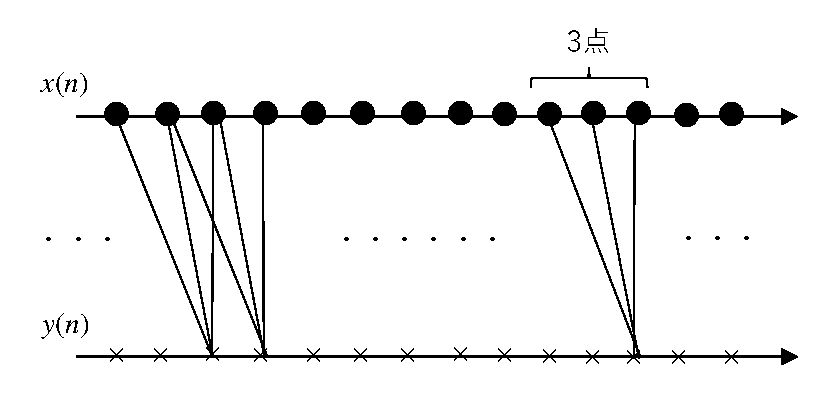
\includegraphics[width=5cm]{fig/zu-2-1.eps}
\end{center}
\caption{3点平均の処理システム}
\label{fig:zu4-2-1}
\end{figure}
式(\ref{eqn:eqn2-1})については,
\begin{enumerate}
	\item 各信号値の加算:$x(n)+x(n-1)+x(n-2)$

	\item 定数値の乗算:1/3を掛けること

	\item 過去の信号値を記憶し遅延させること:$x(n-1)$と$x(n-2)$の扱い
\end{enumerate}
が組み合わさったものである.

この信号処理システムでは,各信号値の加算,定数値1/3の乗算,過去の信号値を記憶して遅延させる,という3種類の演算を用いている.この特徴は,この3点平均の処理システムだけでなく,後述のシステムでも成立する.

\subsection{処理による結果のちがい}

図\ref{fig:zu4-2-2}(a)は,雑音を含んだ正弦波信号を示したものである.この信号に対して先述の3点平均を行った結果が図\ref{fig:zu4-2-2}(b)である.また,図\ref{fig:zu4-2-2}(c)は9点平均を行った結果を示している.3点平均も9点平均もともに雑音の低減がなされていること,特に,9点平均のほうが3点平均よりも雑音の低減効果が高いことがわかる.ところが,信号の大きさが変わり,位相が大きくずれていることも併せてわかる.このことから,
\begin{itemize}
\item 平均処理によって,信号の大きさが変わり,位相がずれる.
\item 平均回数と,信号の大きさの変動と,位相のずれとの関係.
\item 平均回数と雑音の低減効果の関係.
\item 平均処理より,効果的な雑音の除去.
\end{itemize}
に関する疑問が発生するため,これらの疑問点を解決しながら,その処理を実際に行う信号処理システムを説明する.

\begin{figure}[H]
\begin{center}
\begin{minipage}{.35\textwidth}
\begin{center}
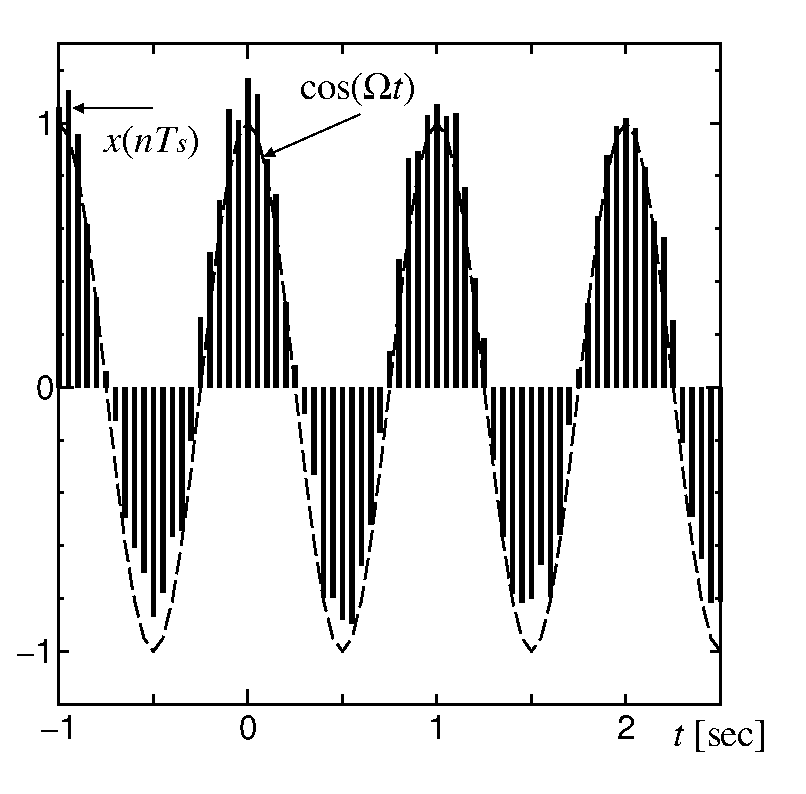
\includegraphics[width=.85\textwidth]{fig/zu-2-2-a.eps}

(a) 雑音を含んだ信号
\end{center}
\end{minipage}
\begin{minipage}{.35\textwidth}
\begin{center}
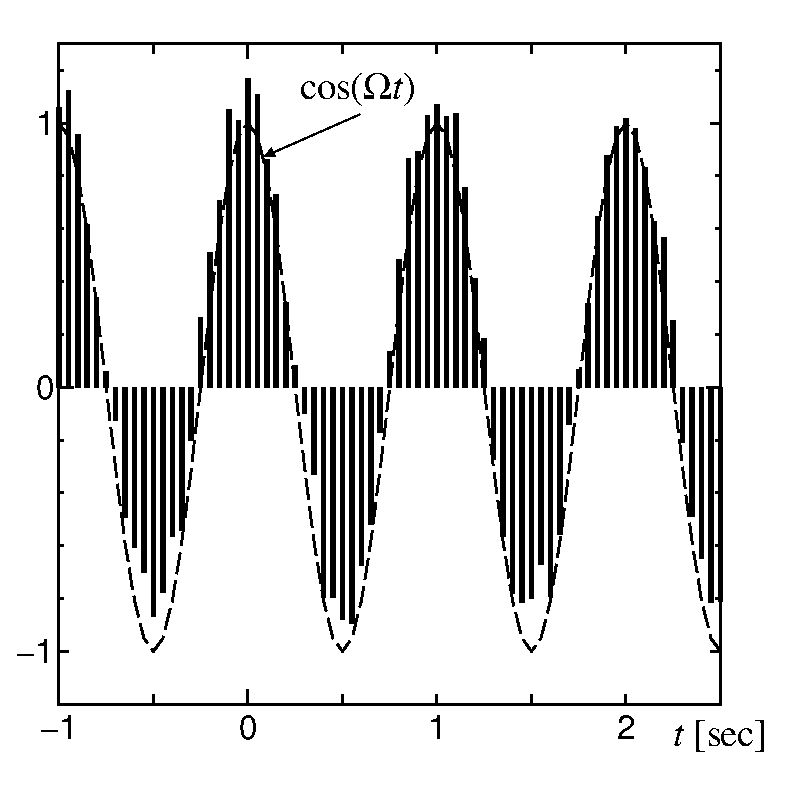
\includegraphics[width=.85\textwidth]{fig/zu-2-2-b.eps}

(b) 3点平均
\end{center}
\end{minipage}
\begin{minipage}{.35\textwidth}
\begin{center}
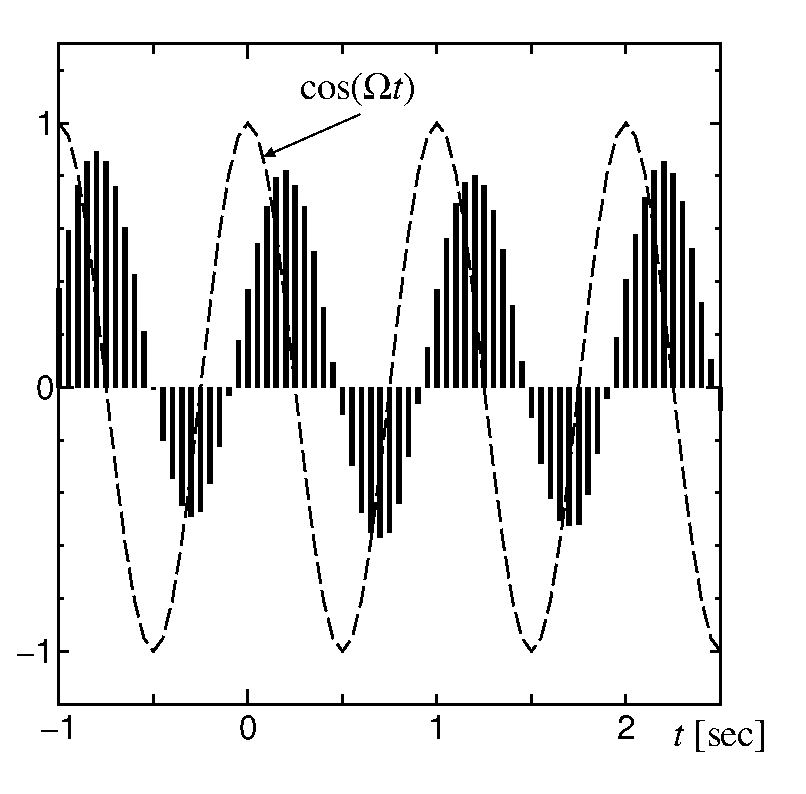
\includegraphics[width=.85\textwidth]{fig/zu-2-2-c.eps}

(c) 9点平均
\end{center}
\end{minipage}
\end{center}\vskip.5\baselineskip
\caption{平均処理による雑音の除去例($F=1$[Hz],$F_s=20$[Hz])}
\label{fig:zu4-2-2}
\end{figure}


\section{信号の例とその性質}

%\subsection{代表的な信号の例}

%以下に示す信号の表現は,1章に述べた正規化表現である.


\subsection{正弦波}

次式で表される信号は正弦波信号である.
\begin{equation}
x(n)=\sin (n\omega)
\end{equation}
または
\begin{equation}
x(n)=\cos (n\omega)
\end{equation}

ここで$\omega$は正規化角周波数である.先述のように,$\omega=\Omega T_s$の関係から,アナログ正弦波信号をサンプリング周期$T_s$でサンプリングしたものと考えてよい.

\subsection{複素正弦波信号}

複素正弦波信号は,次式のように,複素平面上では半径1の単位円として表現されるものである.
\begin{equation}
x(n)=e^{j\omega n}=\cos (\omega n ) +j \sin (\omega n)
\end{equation}
この信号は$j=\sqrt{-1}$を含むため,複素数である.この式はオイラーの公式と呼ばれる関係でもある.

\subsection{単位ステップ信号 $u(n)$}

単位ステップ信号は,図\ref{fig:zu4-2-30}で示されるように,$n \leq 0$で1となるような信号である.
\begin{equation}
u(n) = \left \{ 
\begin{array}{cc}
1, & n \geq 0 \\
0, & n < 0
\end{array}
\right .
\end{equation}

\begin{figure}[H]
\begin{center}
\begin{minipage}{.48\textwidth}
\begin{center}
%\includegraphics[width=9cm]{fig/zu-2-4.eps}
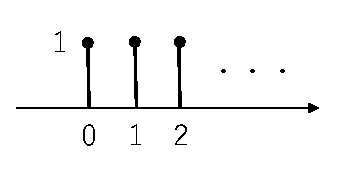
\includegraphics[width=.95\textwidth]{fig/zu-2-4-b.eps}

%(a) 単位ステップ信号 $u(n)$
\end{center}
\end{minipage}
%\begin{minipage}{.48\textwidth}
%\begin{center}
%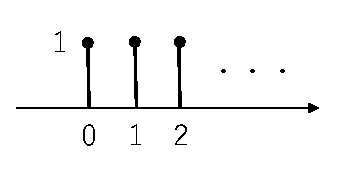
\includegraphics[width=4.8cm]{fig/zu-2-4-b.eps}

%(b) インパルス $\delta(n)$
%\end{center}
%\end{minipage}
\end{center}
%\caption{単位ステップ信号$u(n)$と単位サンプル信号$\delta(n)$}
\caption{単位ステップ信号$u(n)$}
\label{fig:zu4-2-30}
\end{figure}



\subsection{単位サンプル信号(インパルス) $\delta (n)$}

単位サンプル信号は,図\ref{fig:zu4-2-31}に示すように.$n=0$となるところだけ値が1をとり,他が0となる信号である.
\begin{equation}
\delta (n) = \left \{ 
\begin{array}{cc}
1, & n = 0 \\
0, & n \neq 0
\end{array}
\right .
\end{equation}

\begin{figure}[H]
\begin{center}
\begin{minipage}{.48\textwidth}
\begin{center}
%\includegraphics[width=9cm]{fig/zu-2-4.eps}
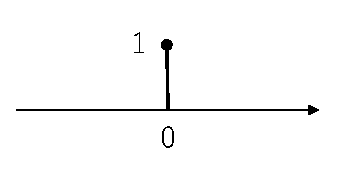
\includegraphics[width=.95\textwidth]{fig/zu-2-4-a.eps}

%(a) 単位ステップ信号 $u(n)$
\end{center}
\end{minipage}
%\begin{minipage}{.48\textwidth}
%\begin{center}
%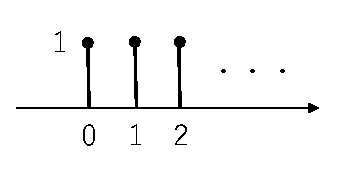
\includegraphics[width=4.8cm]{fig/zu-2-4-b.eps}

%(b) インパルス $\delta(n)$
%\end{center}
%\end{minipage}
\end{center}
%\caption{単位ステップ信号$u(n)$と単位サンプル信号$\delta(n)$}
\caption{単位ステップ信号$u(n)$}
\label{fig:zu4-2-31}
\end{figure}


この単位サンプル信号のことを別名でインパルスとも呼ぶ.ここで$\delta$はギリシャ文字のデルタの小文字である.


ところで,図\ref{fig:zu4-2-4}(a)に示すように$\delta(n-2)$であれば,インパルスの定義から,括弧内の$n-2$が0となるところだけが1で,それ以外が0となる.

もし,次式のような信号の場合であれば,図\ref{fig:zu4-2-4}(b)のように描くことができる.
\begin{equation}
x(n)=-\delta(n+1)+2\delta(n)+\delta(n-2)
\label{eqn:eqn-2-6}
\end{equation}

\begin{figure}[H]
\begin{center}
\begin{minipage}{.3\textwidth}
\begin{center}
%\includegraphics[width=9cm]{fig/zu-2-3.eps}
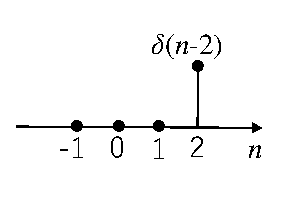
\includegraphics[width=.95\textwidth]{fig/zu-2-3-a.eps}

(a)
\end{center}
\end{minipage}
\begin{minipage}{.3\textwidth}
\begin{center}
%\includegraphics[width=9cm]{fig/zu-2-3.eps}
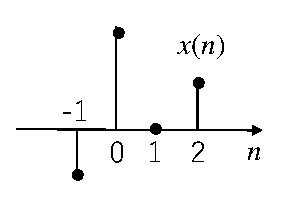
\includegraphics[width=.95\textwidth]{fig/zu-2-3-b.eps}

(b)
\end{center}
\end{minipage}
\begin{minipage}{.3\textwidth}
\begin{center}
%\includegraphics[width=9cm]{fig/zu-2-3.eps}
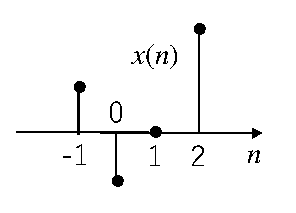
\includegraphics[width=.95\textwidth]{fig/zu-2-3-c.eps}

(c)
\end{center}
\end{minipage}
\end{center}\vskip.5\baselineskip
\caption{インパルス$\delta(n)$の性質}
\label{fig:zu4-2-4}
\end{figure}


この例からわかるように,任意の信号$x(n)$を,インパルス$\delta(n)$の時間$n$をシフトして大きさに重みを付けて加えることによって,表現することができる.
%
つまり,次式のように書くことができる\footnote{たたみ込みの式(\ref{eqn:eqn-2-7})は,積分の形で書き表すと$x(t)=\int_{-\infty}^{\infty}x(t)\delta(\tau - t)dt$
のような形式であり,$x(t)$,$\delta(t)$ともに離散時間信号であるため,式(\ref{eqn:eqn-2-7})に帰着する.
}.
\begin{equation}
x(n)=\sum_{k=-\infty}^{\infty}x(k)\delta(n-k), \hspace{1cm} x(n):任意の信号
\label{eqn:eqn-2-7}
\end{equation}
この式(\ref{eqn:eqn-2-6})と式(\ref{eqn:eqn-2-7})とを比較すると,
\begin{equation}
x(n)=x(-1)\delta(n+1)+x(0)\delta(n)+x(2)\delta(n-2)
\label{eqn:eqn-2-8}
\end{equation}
と書けることから,$x(-1)=-1$,$x(0)=1$,$x(2)=2$であることもわかる.
すなわち,$x(-1)$,$x(0)$,$x(2)$以外では0の値をとることも併せてわかる.


このように,任意の信号$x(n)$を表現できるというインパルスの性質は,これから後の説明を理解する上で重要なことである.


\section{線形時不変システム}

信号処理システムにおいて最も重要なシステムは,線形時不変システムである.この線形時不変システムには,先述の3点平均の計算も含まれる.ここでは,線形時不変システムの概要,その表現法,重要性について説明する.

\subsection{線形性と時不変性}

信号処理システムは,入力信号$x(n)$を他の信号$y(n)$に変換するものと考えることができる.そこで,図\ref{fig:zu4-2-5}に示すようにシステムを入力信号$x(n)$を出力信号$y(n)$に一意的に変換できるものと定義して,その関係を変換(transform)という意味で,
\begin{equation}
y(n)=T[x(n)]
\end{equation}
と表すものとする.変換に際して,その拘束条件によって,システムを時不変システム,線形システムに分類することができる.

\begin{figure}[H]
\begin{center}
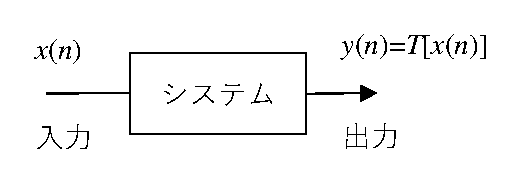
\includegraphics[width=9cm]{fig/zu-2-5.eps}
\end{center}
\caption{線形システムの一般的表現}
\label{fig:zu4-2-5}
\end{figure}

\subsubsection{時不変システム(シフト不変システム)}

\index{じふへんしすてむ@時不変システム}時不変システム(time-invariant system)は,シフト不変システム\index{しふとふへんしすてむ@シフト不変システム}(shift-invariant system)ともいわれる.これは,ある入力$x(n)$に対応する出力を$y(n)$とするときに次式の関係が成立するシステムである.
\begin{equation}
y(n-k)=T[x(n-k)]
\label{eqn:eqn-k2-10}
\end{equation}
ただし,$k$は任意の整数である.

これを図\ref{fig:zu4-2-6}(a)の例を用いて具体的に説明する.図\ref{fig:zu4-2-6}(a)において,信号$x_1(n)$をシステムに入力した場合に出力$y_1(n)$が得られると仮定する.時不変システムでは,図\ref{fig:zu4-2-6}(b)のように入力が$x_2(n)=x_1(n-1)$すなわち時間方向に1だけシフトした場合には,同じ時間だけシフトした$y_2(n)=y_1(n-1)$が出力されるのである\footnote{この線形システムで述べる入力$x_1(n)$,$x_2(n)$は,時不変システムにおける$x_1(n)$,$x_2(n)$と必ずしも同じ関数であるとは限らず,あくまでも任意の関数である.
}.


\subsubsection{線形システム}

線形システム(linear system)とは,任意の入力$x_1(n)$,$x_2(n)$に対応する出力をそれぞれ$y_1(n)=T[x_1(c)]$,$y_2(n)=T[x_2(n)]$とするとき,任意の定数$a$,$b$に対して,次式のような関係が成立するシステムである.

\begin{eqnarray}
T[ax_1(n)+bx_2(n)]&=&T[ax_1(c)]+bT[ax_2(n)] \nonumber \\
 &=&aT[x_1(c)]+bT[x_2(n)] \nonumber \\
 &=&ay_1(n)+by_2(n)
\label{eqn:eqn-2-11}
\end{eqnarray}

\begin{figure}[H]
\begin{center}
%\includegraphics[width=7cm]{fig/zu-2-6.eps}
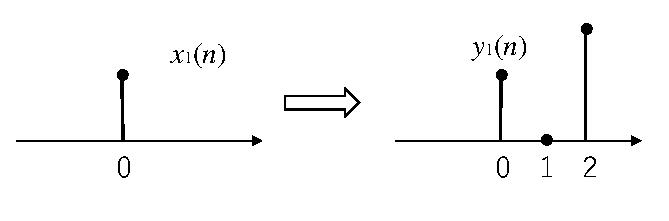
\includegraphics[width=7cm]{fig/zu-2-6-a.eps}

(a)

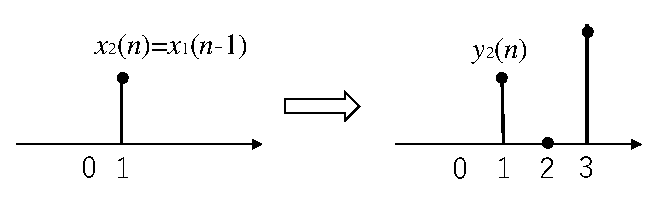
\includegraphics[width=7cm]{fig/zu-2-6-b.eps}

(b)

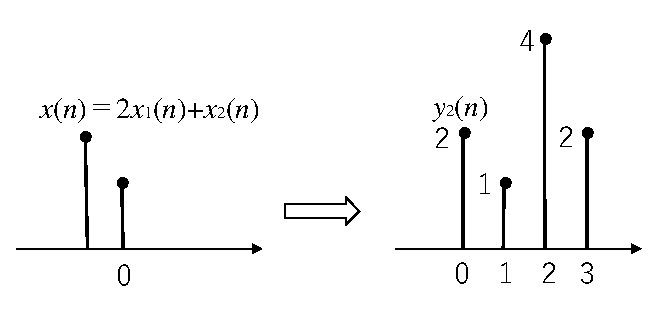
\includegraphics[width=7cm]{fig/zu-2-6-c.eps}

(c)
\end{center}\vskip.5\baselineskip
\caption{システムの入出力の例}
\label{fig:zu4-2-6}
\end{figure}

このことを図\ref{fig:zu4-2-6}(c)を用いて具体的に説明する.図\ref{fig:zu4-2-6}(c)における入力$x(n)$は,次式のように$x_1(n)$と$x_2(n)$を用いて表現される.
\begin{equation}
x(n)=2x_1(n)+x_2(n)
\label{eqn:eqn-k2-11}
\end{equation}
線形システムにおいては,$2x_1(n)$に対する出力$T[2x_1(n)]$は,$y_1(n)$の2倍となる.それを式で示すと,以下のようになる.

\begin{eqnarray}
T[2x_1(n)]&=&2T[x_1(n)] \nonumber \\
 &=&2y_1(n)
\end{eqnarray}\vskip.3\baselineskip

\noindent また,
\begin{equation}
y_2(n)=T[x_2(n)]
\end{equation}
であることから,出力$y(n)$は個々の出力$y_1(n)$,$y_2(n)$の線形和となる次式のように表される.
\begin{equation}
y(n)=2y_1(n)+y_2(n)
\end{equation}

\subsubsection{線形時不変システム}

線形時不変システム(linear time-invariant system)は,時不変性(式(\ref{eqn:eqn-k2-10}))と線形性(式(\ref{eqn:eqn-k2-11}))の条件を同時に満足するシステムのことである.

ただし,時不変性の条件と線形性の条件とはそれぞれ独立な条件であるため,どちらかの条件しか満足しないシステムも存在する.

\subsubsection{因果性システム}

因果性システム(causual system)とは,任意の時刻$n_0$における出力$y(n_0)$が,その時刻より過去の時刻$n\leq n_0$だけの入力$x(n)$を用いて計算されるシステムである.

特に,時系列として与えられるデータを次々に処理して出力する実時間システム(real-time system)の実現のためには,システムの因果性を満足することが重要である.

たとえば,
\begin{equation}
y(n)=\frac{1}{3}\{ x(n) + x(n-1) +x(n-2) \}
\end{equation}
は因果性システムとなるが,
\begin{equation}
y(n)=\frac{1}{3}\{ x(n+1) + x(n) +x(n-1) \}
\end{equation}
は因果性システムではない.

\subsection{インパルス応答とたたみ込み}

\subsubsection{インパルス応答}

線形時不変システムでは,システムにインパルス$\delta(n)$を入力した場合,出力がわかると,任意の入力に対する出力を求めることができる.インパルスを入力した場合の出力$h(n)$を
\begin{equation}
h(n)=T[\delta(n)]
\end{equation}
と書き,この出力$h(n)$をインパルス応答と呼ぶ.

\subsubsection{たたみ込み}

線形時不変システムでは,任意の入力$x(n)$とそれに対応する出力$y(n)$との関係を,
\begin{equation}
y(n)=\sum_{k=-\infty}^{\infty}x(k)h(n-k)
\label{eqn:tata-00}
\end{equation}
と表すことができる.

つまり,任意の入力$x(n)$とそれに対応する出力$y(n)$との関係は,インパルス応答からなるたたみ込みの計算によって導出される.このたたみ込み式を導出するにあたっては,線形性と時不変性の条件が必要である.まず,システムの入出力関係については,
\begin{equation}
y(n)=T[x(n)]
\end{equation}
とおくことができるので,
\begin{equation}
x(n)=\sum_{k=-\infty}^{\infty}x(k)\delta(n-k), \hspace{1cm} x(n):任意の信号
\end{equation}
を代入すると,
\begin{equation}
y(n)=T[\sum_{k=-\infty}^{\infty}x(k)\delta(n-k)]
\label{eqn:eqn-k2-20}
\end{equation}
である.ここで,線形性と時不変性の仮定は特段必要ない\footnote{式(\ref{eqn:eqn-2-11})のように,
\begin{eqnarray}
 T[ax_1(n)+bx_2(n)] 
 = T[ax_1(c)]+T[bx_2(n)] 
 = aT[x_1(c)]+bT[x_2(n)] \nonumber
\end{eqnarray}
のような展開が式(\ref{eqn:tata-01})~式(\ref{eqn:tata-02})で行われている.ここで,$x(k)$は定数であることから変換$T$の外に出すことができる.}.
次に線形性を仮定すると,式(\ref{eqn:eqn-k2-20})は,

\begin{eqnarray}
y(n)&=&T[\sum_{k=-\infty}^{\infty}x(k)\delta(n-k)] \label{eqn:tata-01}\\
 &=&  T[ \cdots + x(0)\delta(n)+ x(1)\delta(n-1)+ \cdots ] \\
 &=& \cdots + T[x(0)\delta(n)]+T[x(1)\delta(n-1)]+ \cdots \\
 &=&\sum_{k=-\infty}^{\infty}T[x(k)\delta(n-k)] \label{eqn:tata-02} \nonumber \\
 &=&\sum_{k=-\infty}^{\infty}x(k)T[\delta(n-k)] \label{eqn:tata-03}
\end{eqnarray}\vskip.3\baselineskip

\noindent さらに,時不変性を仮定する.インパルス応答は,
\begin{equation}
h(n)=T[\delta(n)]
\end{equation}
であるが,時不変性により,
\begin{equation}
h(n-k)=T[\delta(n-k)]
\end{equation}
が成立する.これを式(\ref{eqn:tata-03})に代入すると,

\begin{eqnarray}
y(n)&=&\sum_{k=-\infty}^{\infty}x(k)T[\delta(n-k)] \nonumber \\
 &=&\sum_{k=-\infty}^{\infty}x(k)h(n-k) \label{eqn:tata-04}
\end{eqnarray}\vskip.3\baselineskip

\noindent となるため,式(\ref{eqn:tata-00})のたたみ込みの式が示されたことになる.

\section{システムの実現}

ここでは,たたみ込みを計算する方法について述べることとする.どの方法でも線形時不変システムを実現できる.

\subsection{たたみ込みの計算法}

図\ref{fig:zu4-2-6}の入力信号$x(n)$と出力信号$y(n)$との関係について,出力信号$y(n)$は入力信号$x(n)$とインパルス$h(n)$のたたみ込みによって得られることを説明する.

\subsubsection{入力信号$x(n)$で分割する}

入力信号は,
\begin{equation}
x(n)=2\delta(n)+\delta(n-1)
\end{equation}
のように2つのインパルスを用いているので,個々の信号に対する出力を求めて,その結果を加算すればよい.その結果,

\begin{eqnarray}
y(n)&=&T[2\delta(n)+\delta(n-1)] \nonumber \\
 &=&2T[\delta(n)]+T[\delta(n-1)] \nonumber \\
 &=&2h(n)+h(n-1) \label{eqn:eqn-2-22}
\end{eqnarray}\vskip.3\baselineskip

\noindent となる.

\subsubsection{たたみ込みの値を直接計算}
図\ref{fig:zu4-2-6}に示すような入出力関係を持つシステムは
\begin{equation}
y(n)=x(n)+2x(n-2)
\end{equation}
と書くことができるので,各時刻で計算すると,
\begin{equation}
\left \{
\begin{array}{lll}
y(0)=x(0)+2x(-2)=2+0=2 \\
y(1)=x(1)+2x(-1)=1+0=1 \\
y(2)=x(2)+2x(0)=0+2 \times 2=4 \\
y(3)=x(3)+2x(1)=0+2=2 \\
y(4)=x(4)+2x(2)=0+0=0 \\
\cdots
\end{array}
\right .
\end{equation}
となる.この結果も式(\ref{eqn:eqn-2-22})の結果と一致する.

\subsubsection{多項式積としての計算}

ここでは$z$変換を用いる.$x(n)$,$h(n)$を$z$変換して,次式のような多項式を得る.
\begin{equation}
X(z)=2+z^{-1}
\end{equation}
\begin{equation}
H(z)=1+2z^{-2}
\end{equation}
ここで,$y(n)$の$z$変換$Y(z)$は,

\begin{eqnarray}
Y(z)&=&H(z)X(z) \nonumber \\
 &=&(1+2z^{-2})(2+z^{-1}) \nonumber \\
 &=&2+z^{-1}+4z^{-2}+2z^{-3}
\end{eqnarray}\vskip.3\baselineskip

\noindent となる.$z^{-n}$の係数が$y(n)$になるので,
$y(0)=2$,$y(1)=1$,$y(2)=4$,$y(3)=2$であるから,これも式(\ref{eqn:eqn-2-22})の結果と一致する.


\subsection{ハードウェア表現}

線形時不変システムのハードウェア表現について説明する.これは,たたみ込み計算をハードウェア実現することと同じことである.

\subsubsection{演算要素}

たたみ込みは,乗算,加減算,信号のシフトの3種類の演算により実行される.例として,この3種類の演算を行う演算器を図\ref{fig:zu4-2-10}に示す.線形時不変システムは,これらの演算器を用いて実現することができる.

\begin{figure}[H]
\begin{center}
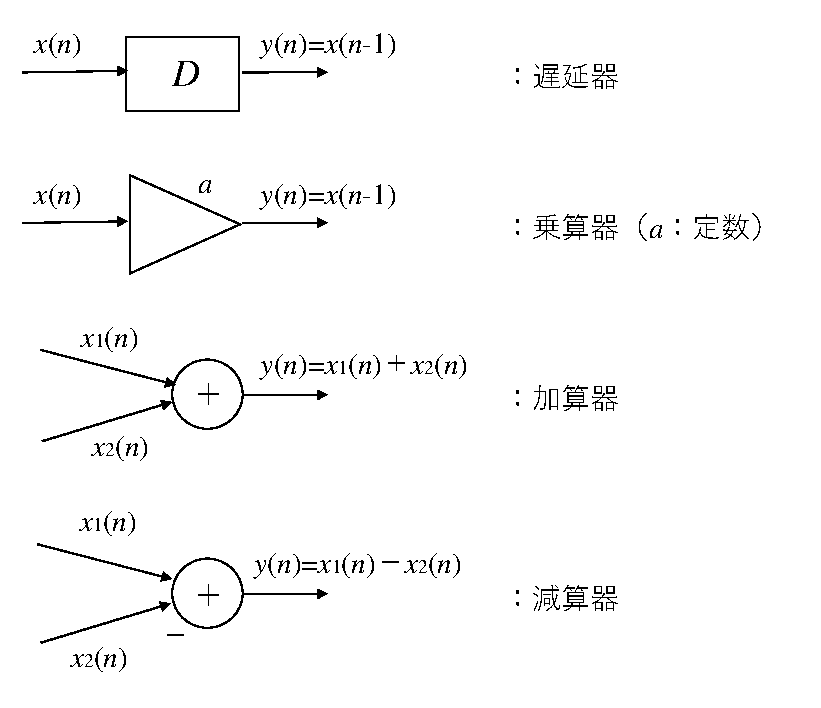
\includegraphics[width=9cm]{fig/zu-2-10.eps}
\end{center}
\caption{システムの演算要素}
\label{fig:zu4-2-10}
\end{figure}


\subsubsection{システムの構成例}

たとえば,次式のようなシステムを考える.
\begin{equation}
y(n)=x(n)+2x(n-2)
\end{equation}
このシステムは図\ref{fig:zu4-2-11}のように構成できる.

\begin{figure}[t]
\begin{center}
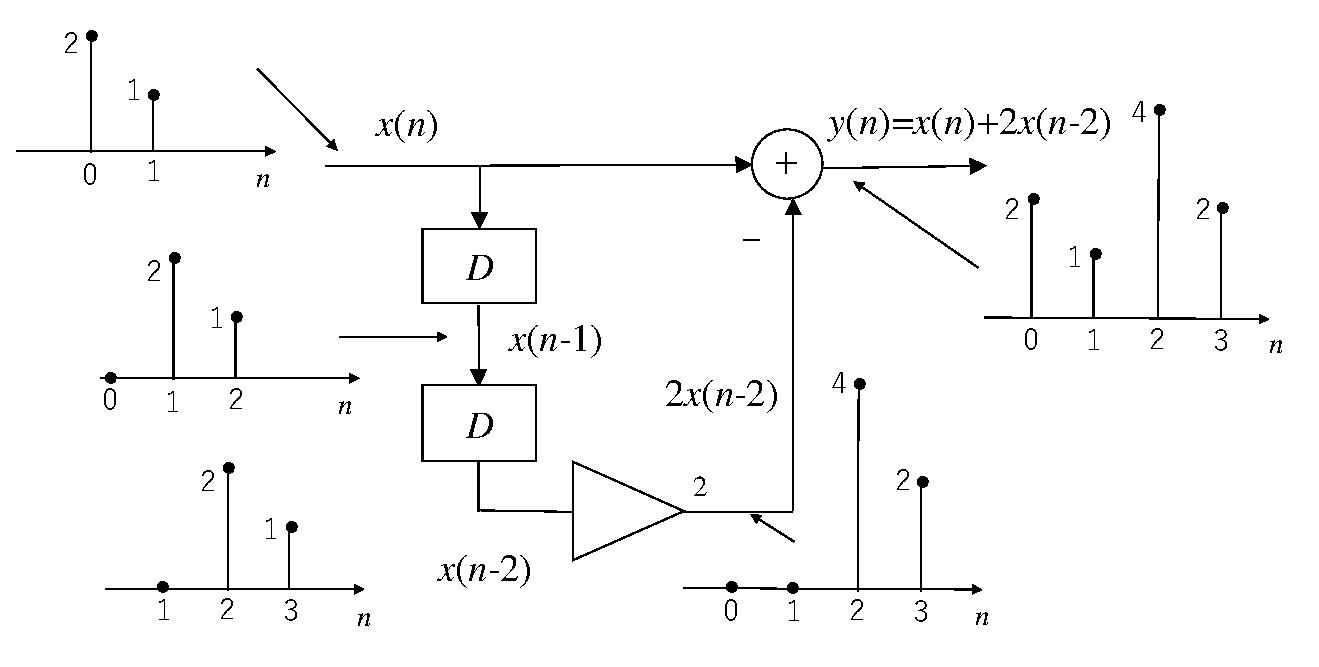
\includegraphics[width=9cm]{fig/zu-2-11.eps}
\end{center}
\caption{システムの構成例}
\label{fig:zu4-2-11}
\end{figure}

これを作図する際のポイントは,以下の3点である.
\begin{itemize}
\item 式からシステムを構成できる.
\item 構成図から式を推定できる.
\item 構成図上の信号の流れがわかる.
\end{itemize}

図\ref{fig:zu4-2-11}のシステムに図\ref{fig:zu4-2-10}の$x(n)$を入力すると,システム各部の信号の流れが示される.このような流れで信号が推移していることがわかる.

\newpage

\subsubsection{システムの一般的な構成例}

一般的なシステムとして次式のようなシステムを考える.
\begin{equation}
y(n)=\sum_{k=0}^{N-1}h(k)x(n-k)
\end{equation}

このシステムは図\ref{fig:zu4-2-12}のように非再帰型システムとして構成される.
ここでは,各乗算器の値がインパルス応答$h(n)$に対応する.


\begin{figure}[H]
\begin{center}
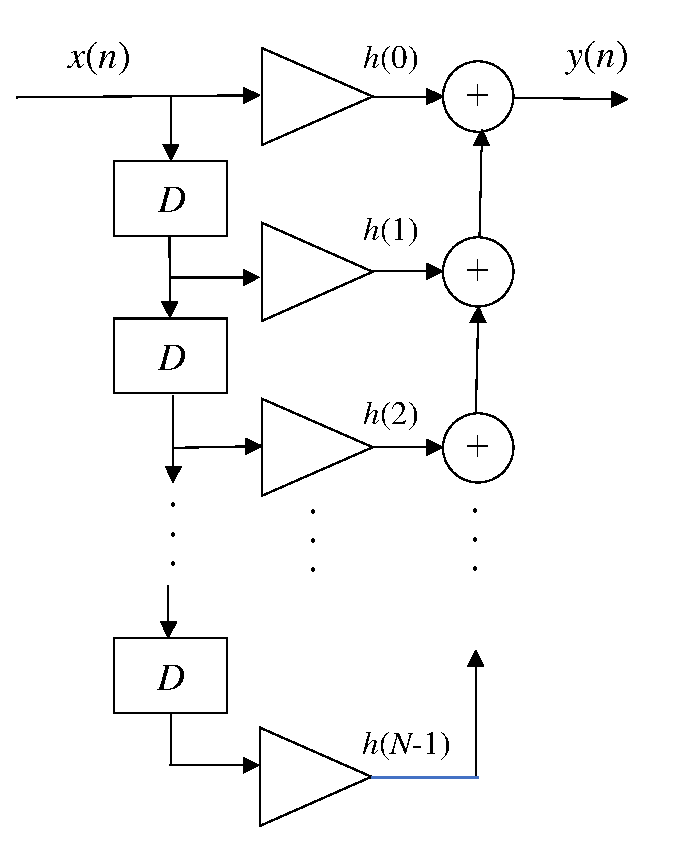
\includegraphics[width=6cm]{fig/zu-2-12.eps}
\end{center}
\caption{システムの構成例}
\label{fig:zu4-2-12}
\end{figure}

システムの構成には自由度があり,ひとつのシステムに対して複数通りのシステムの構成があることから,これ以外の構成法もあるだろうが,それについては別途説明する.



\subsection{フィードバックのあるシステム}

\subsubsection{システムの例}

いま,次式で表されるようなシステムがあるとする.
\begin{equation}
y(n)=x(n)+by(n-1)
\label{eqn:2-30}
\end{equation}
ここで$b$は定数である.この式は右辺に$y(n-1)$があることから,過去の出力を入力に用いて出力するという,いわゆるフィードバックするものであり,たたみ込みではない.

この場合のシステムは図\ref{fig:zu4-2-14}(a)に示されるような構成となり,出力$y(n)$が入力側に戻ることがわかる.このように,ある時刻での出力結果を基に後の出力を求める処理をフィードバック処理といい,フィードバック処理を伴うシステムを再帰型システム(recursive system)という.他方,フィードバック処理のないシステムを非再帰型システム(nonrecursive system)という.

この図\ref{fig:zu4-2-14}(a)の構成から,システムのインパルス応答を求める.入力として$x(n)=\delta(n)$を仮定すると,式(\ref{eqn:2-30})は,

\begin{eqnarray}
y(n)&=&x(n)+by(n-1) \nonumber \\
 &=&x(n)+b(x(n-1)+by(n-2)) \nonumber \\
 &=&x(n)+bx(n-1)+b^2y(n-2) \nonumber \\
 &=&b^0x(n)++bx(n-1)+b^2(x(n-2)+by(n-3)) \nonumber \\
 & & \cdots \nonumber \\
 &=&\sum_{k=0}^{\infty}b^k(n-k) \label{eqn:2-31}
\end{eqnarray}\vskip.3\baselineskip

\noindent のように変形され,たたみ込みの式として表現される.

このことから,図\ref{fig:zu4-2-14}(b)のように時刻$n=0$から,$1,b,b^2,b^3,\cdots$と無限に続くインパルス応答となることがわかる.
%
したがって,このシステムは,式(\ref{eqn:2-30}),式(\ref{eqn:2-31})のいずれの表現でも記述されることがわかる.

\begin{figure}[H]
\begin{center}
\begin{minipage}[b]{.48\textwidth}
\begin{center}
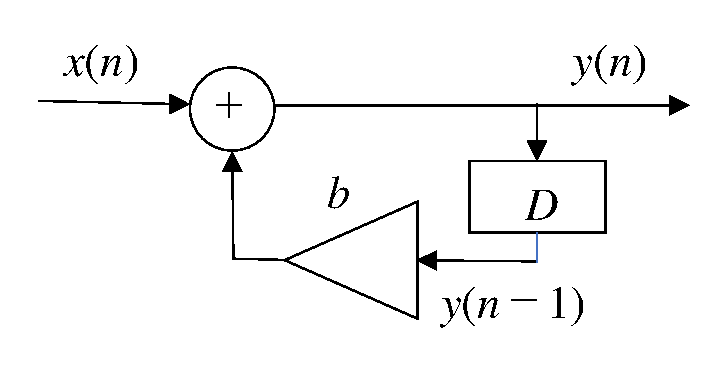
\includegraphics[width=.95\textwidth]{fig/zu-2-14-a.eps}

(a)
\end{center}
\end{minipage}
\begin{minipage}[b]{.48\textwidth}
\begin{center}
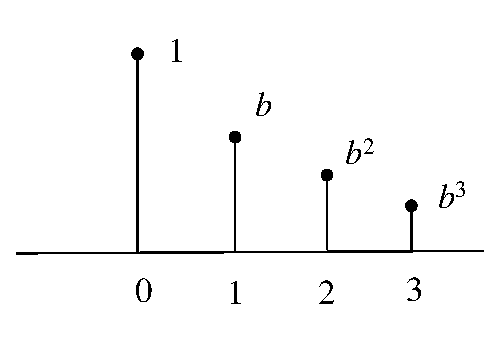
\includegraphics[width=.95\textwidth]{fig/zu-2-14-b.eps}

(b)
\end{center}
\end{minipage}
\end{center}\vskip.5\baselineskip
\caption{フィードバック処理のあるシステムの構成例}
\label{fig:zu4-2-14}
\end{figure}




\subsubsection{フィードバックの必要性}

先述のように,
\begin{equation}
y(n)=x(n)+by(n-1)
\label{eqn:2-30-1}
\end{equation}
をハードウェア実現する際に,
\begin{equation}
y(n)\sum_{k=0}^{\infty}b^k(n-k)
\end{equation}
として考えた場合には,右辺の和が無限個から成り立つので,無限個の演算(乗算,加算,遅延)が必要となってくる.

ところが,式(\ref{eqn:2-30-1})のままシステムを構成すると,図\ref{fig:zu4-2-14}(a)のように有限個の演算により実現可能となる.
%
このように,無限個のインパルス応答を持つシステムは,再帰的型システムとして実現することがあることがわかる.

\subsubsection{IIRシステムとFIRシステム}

システムには,無限個のインパルス応答を持つ無限インパルス応答システム(IIRシステム)と,有限個のインパルス応答を持つ有限インパルス応答システム(FIRシステム)に分類される.

図\ref{fig:zu4-2-14}に示すようなシステムは,式(\ref{eqn:2-31})無限個のインパルス応答から構成されるためIIRシステムであり,図\ref{fig:zu4-2-15}に示すような3点平均を計算するシステムは,3個という有限個のインパルス応答から構成されるためFIRシステムである.

\begin{figure}[H]
\begin{center}
\begin{minipage}[b]{.5\textwidth}
\begin{center}
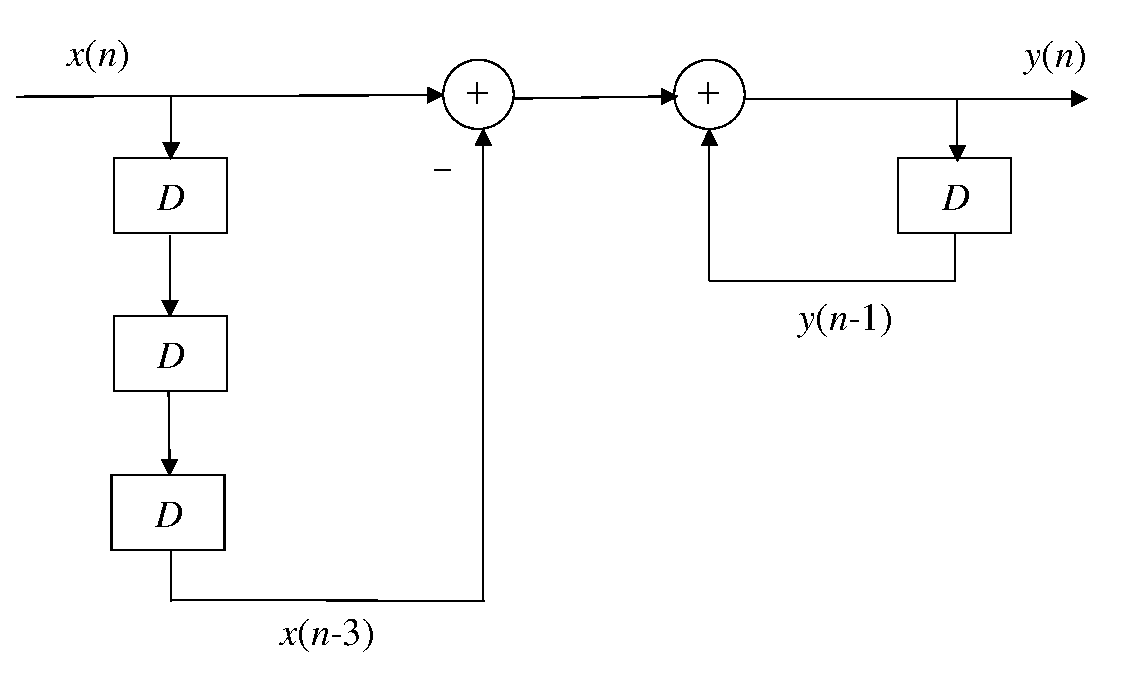
\includegraphics[height=35mm]{fig/zu-2-15a.eps}

(a) 再帰型システム
\end{center}
\end{minipage}
\begin{minipage}[b]{.3\textwidth}
\begin{center}
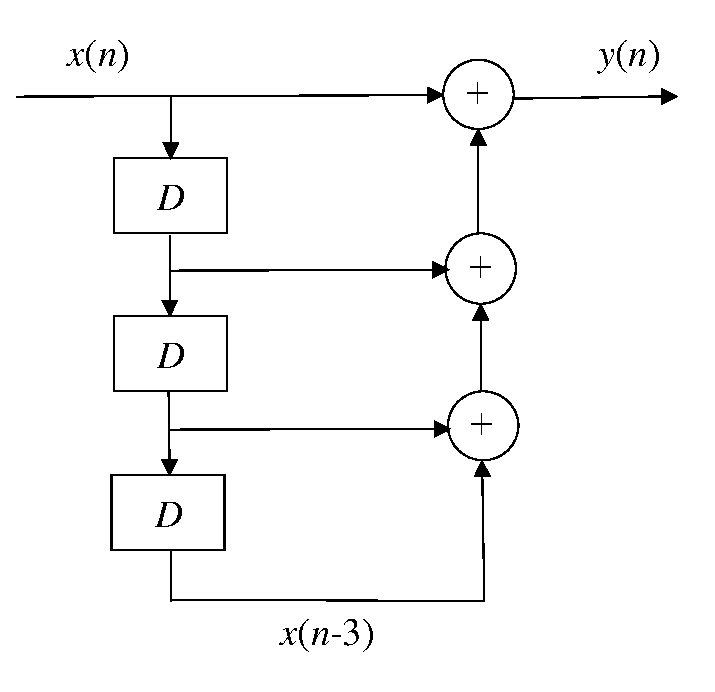
\includegraphics[height=35mm]{fig/zu-2-15b.eps}

(b) 非再帰型システム
\end{center}
\end{minipage}
\end{center}\vskip.5\baselineskip
\caption{システムの構成例}\label{fig:zu4-2-15}
\end{figure}


IIRシステムはフィードバック処理を有するシステムすなわち再帰型システムであるが,再帰的システムは必ずしもIIRシステムであるとは限らない.
%
その一例として,次式で示されるようなシステムについて考察する.
\begin{equation}
y(n)=x(n)-x(n-3)+y(n-1)
\label{eqn:2-30-5}
\end{equation}

この式は,右辺に$y(n-1)$なる出力に遅延を加えたものが存在するため,フィードバック処理を含むものである.ここで,

\begin{eqnarray}
y(n)&=&x(n)-x(n-3)+y(n-1) \nonumber \\
 &=&x(n)-x(n-3)+x(n-1)-x(n-4)+y(n-2) \nonumber \\
 &=&x(n)-x(n-3)+x(n-1)-x(n-4)+x(n-2) \nonumber \\
 & &-x(n-5)+y(n-3) \nonumber \\
 &=&x(n)-x(n-3)+x(n-1)-x(n-4)+x(n-2) \nonumber \\
 & &-x(n-5)+x(n-3)-x(n-6)+y(n-4) \nonumber \\
 &=&x(n)+x(n-1)-x(n-4)+x(n-2)-x(n-5) \nonumber \\
 & &-x(n-6)+x(n-4)-x(n-7)+y(n-5) \nonumber \\
 &=&x(n)+x(n-1)+x(n-2)-x(n-5)-x(n-6) \nonumber \\
 & &-x(n-7)+x(n-5)-x(n-8)+y(n-6) \nonumber \\
 &=&x(n)+x(n-1)+x(n-2)-x(n-6)-x(n-7) \nonumber \\
 & &-x(n-8)+x(n-6)-x(n-9)+y(n-7) \nonumber \\
 &=&x(n)+x(n-1)+x(n-2)-x(n-7)-x(n-8) \nonumber \\
 & &-x(n-9)+x(n-7)-x(n-10)+y(n-8) \nonumber \\
 & & \cdots \nonumber \\
 &=&x(n)+x(n-1)+x(n-2)
\label{eqn:2-30-6}
\end{eqnarray}\vskip.3\baselineskip

\noindent と書き換えることができるため,有限個の処理で済むようなFIRシステムに帰着することがわかる.

このように,IIRシステムはフィードバック処理を有するシステムすなわち再帰型システムであるが,その逆に再帰的システムがIIRシステムであるとは限らないことが例示された.

\subsection{定係数差分方程式の導入}

線形時不変システムはたたみ込みで表現できることがわかったが,IIRのシステムの実現を行うには,たたみ込みのために無限の演算が対応することが大変厄介な問題であるとされてきた.そこで,定係数差分方程式の概念を用いてIIRシステムを便利に実現できることを説明する.

\subsubsection{定係数差分方程式}

ここでは,システムの入出力の関係が次式で表されるものと考える.
\begin{equation}
y(n)=\sum_{k=0}^{M}a_kx(n-k)+\sum_{k=1}^{N}b_ky(n-k)
\label{eqn:2-32}
\end{equation}
この表現を定係数差分方程式と呼ぶ.ここで,$a_k$, $b_k$はそれぞれ定数である.
%
なお,式(\ref{eqn:2-30-1})として示した
\begin{equation}
y(n)=x(n)+by(n-1)
\label{eqn:2-30-11}
\end{equation}
は,定係数差分方程式の特殊な場合に相当する\footnote{定係数差分方程式の特殊な場合として式(\ref{eqn:2-30-11})については,式(\ref{eqn:2-32})における,$M=0$,$N=1$なる場合である.}.


たたみ込み表現では,無限個のインパルス応答$h(n)$を用いて入出力関係を記述している.しかしながら,この定係数差分方程式では,有限個の係数$a_k$および$b_k$で記述され,右辺に出力$y(n-k)$が加えられる点が異なる.このことから,フィードバックを含めることができるという意味から,IIRシステムを有限に表現することが可能である.

\subsubsection{初期休止条件}

初期休止条件の概念を理解するために,式(\ref{eqn:2-30-11})のインパルス応答を求めてみる.まず,入力について$x(n)=\delta(n)$を仮定し,$n=0$を代入すると,
\begin{equation}
y(0)=\delta(0)+by(-1)
\end{equation}
となる.$y(-1)$は入力を加える前の出力の初期状態を意味する.ここで,$y(-1)=0$を仮定すると,
\begin{equation}
\left \{
\begin{array}{lll}
y(0)&=&x(0)+by(-1)=1+0=1 \\
y(1)&=&x(1)+by(0)=0+b\times 1=b \\
y(2)&=&x(2)+by(1)=0+b\times b=b^2 \\
 & & \cdots
\end{array}
\right .
\end{equation}
と応答を求めることができるので,$y(-1)=0$であるとすれば,
\begin{equation}
y(n)=b^n
\end{equation}
と書くことができる.ここでは$y(0)=0$と仮定していたが,一般的に$y(0)\neq 0$である場合については,$y(-1)=c$とおくと,
\begin{equation}
\left \{
\begin{array}{ccl}
y(0)&=&x(0)+by(-1)=x(0)+c=x(0)+c \\
y(1)&=&x(1)+by(0)=0+b(x(0)+c)=b(x(0)+c) \\
y(2)&=&x(2)+by(1)=0+b^2(x(0)+c)=b^2(x(0)+c) \\
 & & \cdots \\
y(n)&=&b^n(x(0)+c)
\end{array}
\right .
\end{equation}
となる.

このように,$c=0$であれば$y(0)$の大きさは$x(0)$の大きさに比例することから線形時不変システムに対応するが,$c\neq 0$であれば$y(0)$の大きさは$x(0)$の大きさに比例しないことから線形時不変システムに対応しないことがわかる.

しかしながら,線形時不変システムの記述法のひとつとして,定係数差分方程式を用いる場合には,一定の条件が必要となる.その条件とは,時刻$n<n_0$において$x(n)=0$ならば,時刻$n<n_0$において$y(n)=0$となることが常に仮定されることである.この条件を初期休止条件 (initial rest condition) と呼ぶ.この条件の下で,定係数差分方程式は線形定係数差分方程式と呼ばれるのである.

\subsubsection{差分方程式の構成}

次式に示すような線形定係数差分方程式についてシステムを構成する.
\begin{equation}
y(n)=\sum_{k=0}^{M}a_kx(n-k)+\sum_{k=1}^{N}b_ky(n-k)
\label{eqn:2-32-2}
\end{equation}
この式でも,乗算,加減算,信号のシフト,の3種類の演算から構成されることから,図\ref{fig:zu4-2-16}のようなシステムの構成を得ることができる\footnote{この線形定係数差分方程式をシステムに表す場合には,自由度があるという理由から,図\ref{fig:zu4-2-16}以外の構成も考えることができる.その議論は後の章で述べる.}.

\begin{figure}[H]
\begin{center}
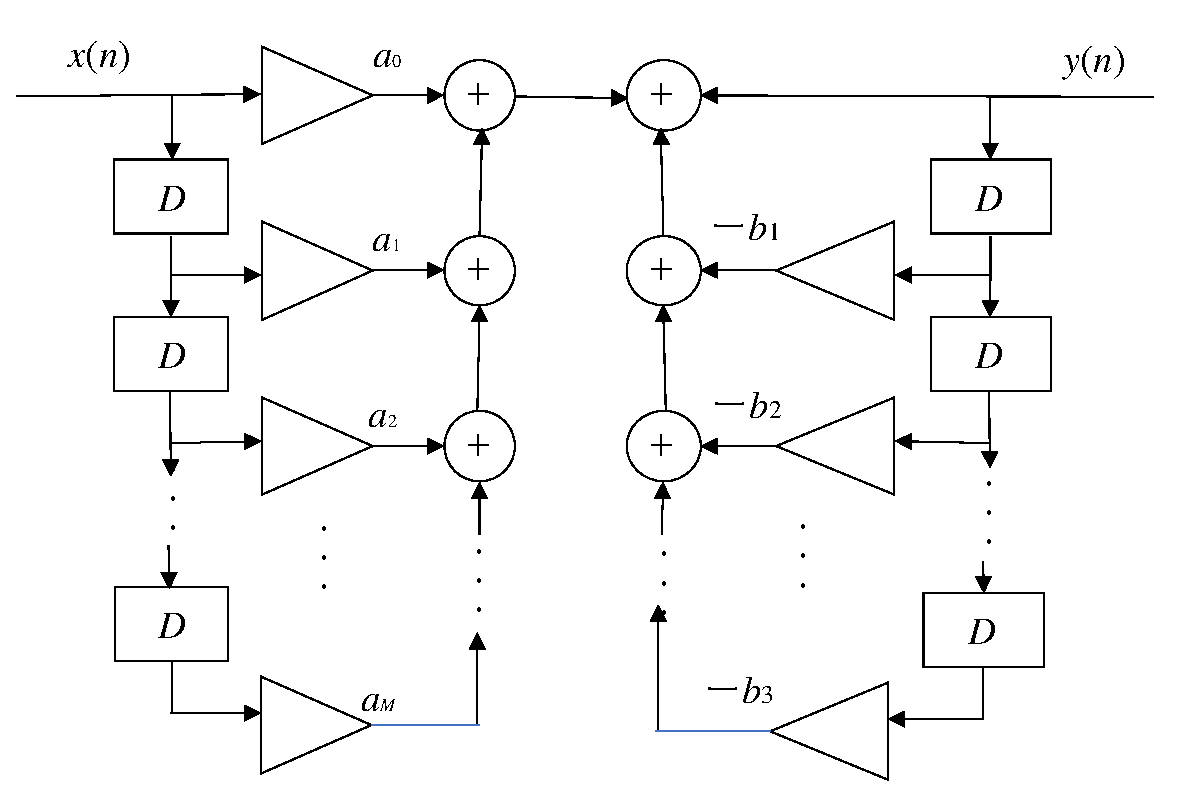
\includegraphics[width=8cm]{fig/zu-2-16.eps}
\end{center}
\caption{差分方程式の構成}
\label{fig:zu4-2-16}
\end{figure}

\section{システムの因果性と安定性の判別}

線形時不変システムのあらゆる性質は,すべてインパルス応答$h(n)$によって記述される.ここでは,インパルス応答を用いたシステムの因果性ならびに安定性の判別法を説明する.

\subsection{因果性システム}

因果性システムとは,ある時刻$n$での出力$y(n)$を求めるために,時刻$n$より未来の入力を必要としないシステムのことである.

線形時不変システムが因果性を満たすための必要十分条件は,
\begin{equation}
h(n)=0, \hspace{1cm} n<0
\end{equation}
である.つまり,負の時間(未来)でインパルス応答の値が0であればよい.


この必要十分条件について,十分条件とは「この条件を満たせば因果性システムである」ということであり,必要条件とは「この条件を満たさなかったら必ず因果性システムではない」ということである.

ところで,3点平均を求めるシステムについて,
\begin{equation}
y(n)=\frac{1}{3}(x(n)+x(n-1)+x(n-2))
\end{equation}
は,未来の値を含まないため,因果性システムであることがわかるが,
\begin{equation}
y(n)=\frac{1}{3}(x(n+1)+x(n)+x(n-1))
\end{equation}
は,未来の値を含むため,因果性システムではないことがわかる.

\subsection{安定なシステム}

安定なシステムとは,有限な値を持つ任意の入力信号をシステムに加えたとき,出力の値が必ず有限となるシステムである.この安定性は,有限入力有限出力安定(Bounded Input Bounded Output Stability:BIBO安定)といわれる.

線形時不変システムがBIBO安定であるための必要十分条件は,インパルス応答が絶対加算可能であること,すなわち,
\begin{equation}
\sum_{n=-\infty}^{\infty}|h(n)| < \infty
\label{eqn:2-36}
\end{equation}
である.

この安定性の条件について証明する.いま,すべての$n$に対して$|x(n)|\leq M$が成立する定数$M$を考える.このとき,たたみ込みの式から,出力$y(n)$の大きさに対して次式が成立する.

\begin{eqnarray}
|y(n)&=&\left | \sum_{k=-\infty}^{\infty}h(k)x(n-k) \right | \nonumber \\
 &\leq& \sum_{k=-\infty}^{\infty}|h(k)||x(n-k)| \nonumber \\
 &\leq& M \sum_{k=-\infty}^{\infty}|h(k)|M \nonumber \\
 &=& M \sum_{k=-\infty}^{\infty}|h(k)|
\end{eqnarray}\vskip.3\baselineskip

ここでは,不等式の性質$|a+b|\leq |a|+|b|$($a$,$b$:定数)を利用している.したがって,式(\ref{eqn:2-36})のもとで,常に
\begin{equation}
|y(n)|< \infty
\end{equation}
が成立し,安定性が保証される.


\subsection{IIRシステムについて}

IIRシステムは,無限のインパルス応答を持つ.したがって,BIBO安定である条件を照らし合わせると,不安定なシステムである可能性があることがわかる.一方,FIRシステムにおいては安定性は保証される.

ところで,改めて式(\ref{eqn:2-30-1})ならびに図\ref{fig:zu4-2-14}に示すようなIIRシステムを考えると,このシステムがBIBO安定条件を満たすかどうかは,乗算器の値$b$によって決まる.すなわち,
\begin{equation}
|b|\geq 1
\end{equation}
である場合には,システムの安定性は満足されず,不安定となる.

図\ref{fig:zu4-2-17}にインパルス応答の例を示しているが,それから因果性,安定性を判定した結果が示されている.このように,インパルス応答を観測するだけで,システムの因果性や安定性を判別することができる.

\begin{figure}[H]
\begin{center}
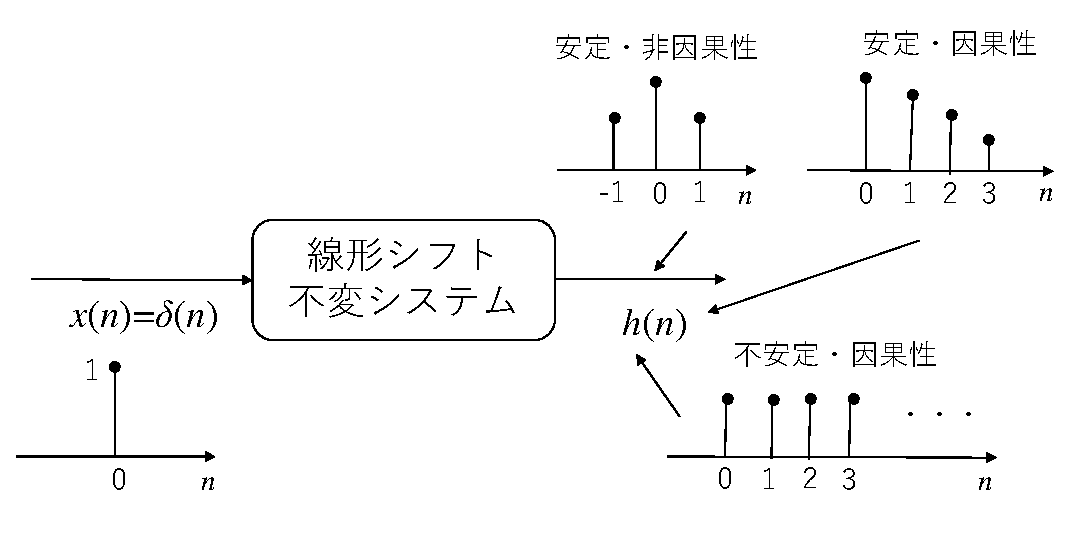
\includegraphics[width=9cm]{fig/zu-2-17.eps}
\end{center}
\caption{因果性,安定性の判別例}
\label{fig:zu4-2-17}
\end{figure}

\section*{演習問題}

\subsection*{問題\ref{chapter:ch-2}.1}

以下のシステムが線形性と時普遍性の条件をそれぞれ満足しているかどうか示せ.

(1) $y(n)=x(n)+x(n-1)+1$

(2) $y(n)=nx(n-1)$

(3) $y(n)=2x(2n-1)$

\subsection*{問題\ref{chapter:ch-2}.2}

システム$y(n)=x(n)-2x(n-1)+x(n-2)$の場合において,以下の問に答えよ.

(1) このシステムのインパルス応答を求めよ.

(2) 単位ステップ信号$u(n)$を加えた場合の出力$y(n)$を求めよ.

(3) このシステムの構成図を示せ.

%\subsection*{問題\ref{chapter:ch-2}.3}

%以下のシステムにおけるハードウェア構成図を示し,インパルス応答を求めよ.

%(1) $y(n)=x(n)+2x(n-1)+3x(n-2)$

%(2) $y(n)=x(n)+2x(n-1)+3y(n-2)$


